% !TeX root = ../build/main.tex

\martai{It is not clear what is the advantage of defining a protocol like this. Is it easy because it is easy to implement as an arithmetic circuit? Make the advantage clear.}

\martai{Yes. The advantage is that we can define many types of voting systems (or recounting) with just these few variables. Moreover, we avoid if-else statements, which makes it very convenient to implement in-circuit. More info here: \url{https://docs.vocdoni.io/architecture/data-schemes/ballot-protocol.html\#vocdoni-results-interpretation} (no multiple question supported).}

\martai{How is the voter's $\weight$ encoded as part of the ballot?}

The \davinci ballot protocol is a simple and efficient mechanism for casting and tallying votes in any type of election or collective decision-making process. Each voting process consists of one or several fields and voters are required to provide a response for each of these fields in their ballot.

The responses in the ballot are represented as a sequence of natural numbers, each corresponding to the voter’s choice for the respective field. Results are accumulated into a single array. Each position in the array corresponds to the sum of all votes cast for that field across all voters.

The ballot protocol is defined by a set of configurable variables that dictate how votes must be cast. This way the protocol can accommodate a wide range of voting processes and behaviors. The list of variables is the following.

\begin{enumerate}
	\item \maxcount: it defines the maximum number of fields in a ballot (max 64).
	\item \maxvalue: it is the maximum allowable value for any field in a ballot (if greater than 0).
	\item \minvalue: it is the minimum allowable value for any field in a ballot (default 0).
	\item \uniquevalues: it specifies whether voters can select the same value multiple times within a ballot (default false).
	\item \maxtotalcost: it limits the sum of all field values in a ballot (if greater than 0).
	\item \mintotalcost: it specifies a minimum required total sum of field values in a ballot (default 0)
	\item \costexponent: it defines the exponent used to calculate the "cost" of votes for each field (default 1).
\end{enumerate}

\martai{"if greater than 0" vs. "default" (make it consistent).}

\begin{figure}[H]
	\centering
	\fbox{
		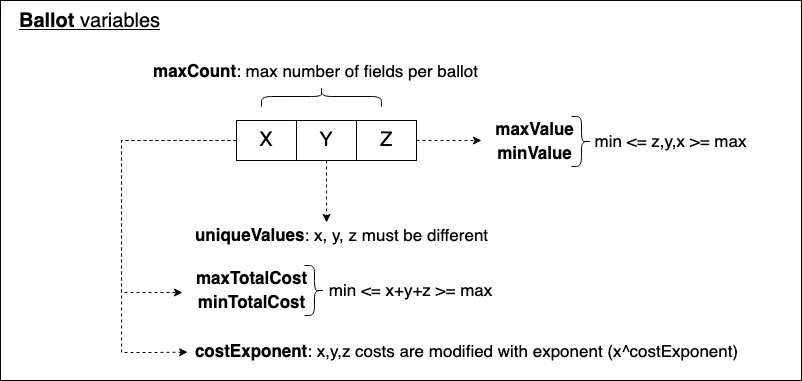
\includegraphics[scale = 0.4, draft = false]{\figs/ballot-variables.png}}
\end{figure}

\martai{In Figure: when is says uniqueValues: x, y, z must be different -- this is if uniqueValues = false, right?}

\paragraph{Example 1: Rating candidates.}

\martai{Reorder names Lennon, Hendrix, Joplin alphabetically.}
\martai{In this example, the rest of variables are default, right? E.g. minValue = 0?}

Consider a voting process where voters are asked to rate three candidates: Lennon, Hendrix, and Joplin. Voters rate each candidate from 0 to 5 stars, and each vote is represented as an array where each position corresponds to the candidate’s rating. The configuration of this voting would be the following:

\begin{itemize}
	\item \maxcount: 3
	\item \maxvalue: 5
	\item \uniquevalues: Yes
\end{itemize}

Ballots:

\begin{itemize}
	\item Vote 1: \texttt{[3, 2, 5]} (3 stars for Lennon, 2 stars for Hendrix, 5 stars for Joplin)
	\item Vote 2: \texttt{[4, 3, 2]}
	\item Vote 3: \texttt{[2, 4, 5]}
\end{itemize}

\martai{I would write 4 ballots.}

After accumulating the votes:

\begin{itemize}
	\item Results Array: \texttt{[3+4+2, 2+3+4, 5+2+5] = [9, 9, 12]}\\
	Lennon received 9 points, Hendrix received 9 points, and Joplin received 12 points.
\end{itemize}

\martai{In the above example, there is no limit to maxTotalCost, right? Maybe add something like, if maxTotalcost = X, then one of the previous ballots would be invalid (and explain why).}

\paragraph{Example 2: Quadratic voting for resource allocation.} 

In a scenario where voters distribute a fixed number of credits across different options (e.g., selecting funding levels for NGOs), the ballot allows voters to assign multiple points, but the cost of casting multiple votes for a single option increases quadratically.

Configuration:

\begin{itemize}
	\item \maxcount: 4
	\item \maxtotalcost: 12 (credits)
	\item \costexponent: 2 (quadratic)
\end{itemize}

Ballots:

\begin{itemize}
	\item Vote 1: \texttt{[2, 2, 2, 0]}
	\item Vote 2: \texttt{[1, 1, 3, 1]}
	\item Vote 3: \texttt{[0, 2, 1, 2]}
\end{itemize}

\martai{Add a fourth vote, e.g. [3, 3, 0, 0]. Then mention that the first 3 ballots are ok because $2^2 + 2^2 + 2^2 = 12$, $1^2 + 1^1 + 3^2 + 1^2 = 12$, $2^2 + 1 + 2^2 = 9 < 12$, but $3^2 + 3^2 = 18 > 12$, and therefore it's invalid. Did I get this right?}


After accumulating the votes:


\begin{itemize}
	\item Results Array: \texttt{[2+1+0, 2+1+2, 2+3+1, 0+1+2] = [3, 5, 6, 3]} \\
	Each position in the array represents the total sum of credits allocated to each NGO.
\end{itemize}

\martai{Cost may be dependant on the voter's weight.}